%# -*- coding: utf-8-unix -*-
%%==================================================
%% thesis.tex
%%==================================================

\documentclass[master, fontset=windows, openright, twoside]{sjtuthesis}
% \documentclass[%
%   bachelor|master|doctor,	% 必选项
%   fontset=adobe|windows,  	% 只测试了adobe
%   oneside|twoside,		% 单面打印,双面打印(奇偶页交换页边距,默认)
%   openany|openright, 		% 可以在奇数或者偶数页开新章|只在奇数页开新章(默认)
%   zihao=-4|5,, 		% 正文字号:小四、五号(默认)
%   review,	 		% 盲审论文,隐去作者姓名、学号、导师姓名、致谢、发表论文和参与的项目
%   submit			% 定稿提交的论文,插入签名扫描版的原创性声明、授权声明 
% ]

% 逐个导入参考文献数据库
\addbibresource{bib/thesis.bib}

\begin{document}

%% 无编号内容:中英文论文封面、授权页
%# -*- coding: utf-8-unix -*-
\title{基于农业物联网和多物理场仿真的智能温室监测与控制研究}
\author{高浩天}
\advisor{黄震宇副教授}
\defenddate{2016年12月17日}
\school{上海交通大学}
\institute{电子信息与电气工程学院}
\studentnumber{1140359026}
\major{仪器仪表工程}

\englishtitle{Greenhouse Monitor}
\englishauthor{\textsc{Gao Haotian}}
\englishadvisor{Associate Prof. \textsc{Huang Zhenyu}}
\englishschool{Shanghai Jiao Tong University}
\englishinstitute{\textsc{School of Electronics and Electric Engineering} \\
  \textsc{Shanghai Jiao Tong University} \\
  \textsc{Shanghai, P.R.China}}
\englishmajor{Instrument}
\englishdate{Dec. 17th, 2016}


\maketitle

\makeenglishtitle

\makeatletter
\ifsjtu@submit\relax
	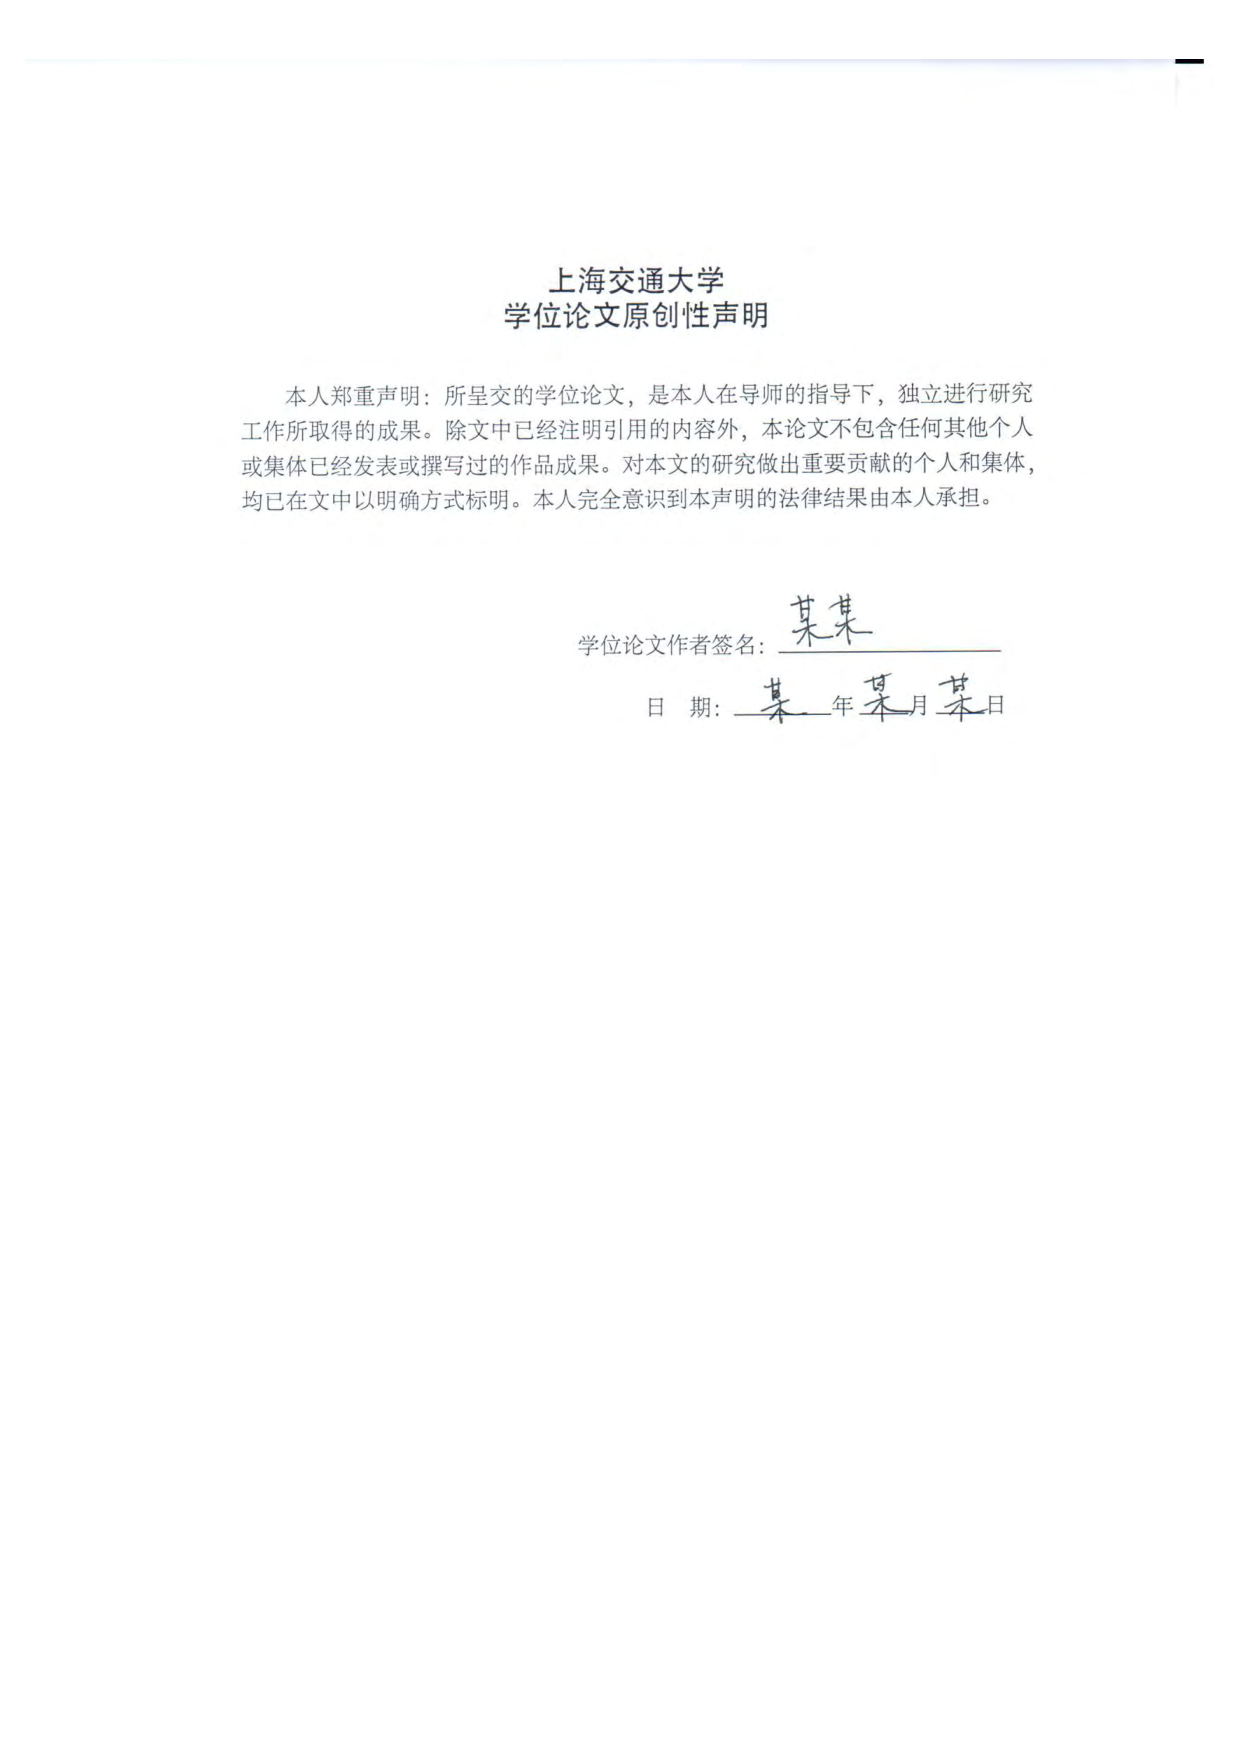
\includepdf{pdf/original.pdf}
	\cleardoublepage
	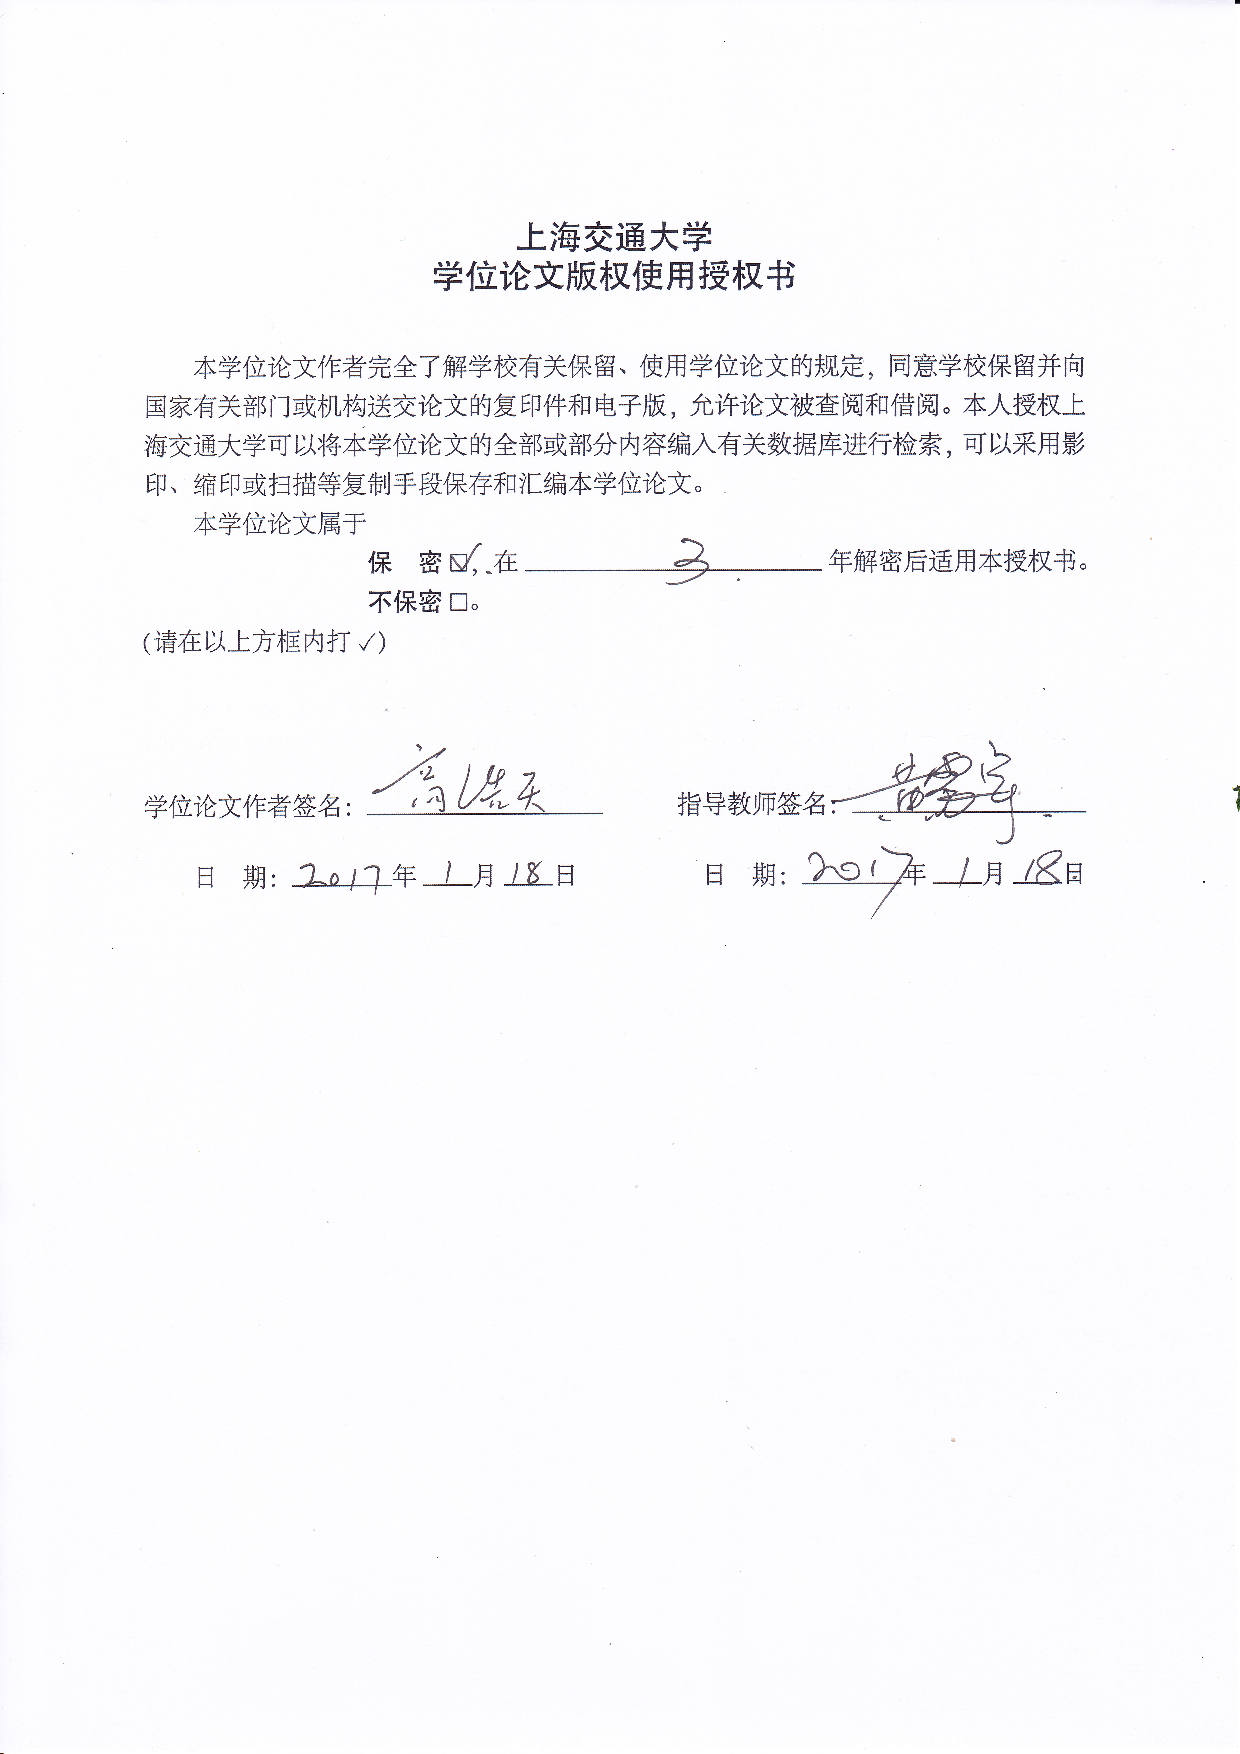
\includepdf{pdf/authorization.pdf}
	\cleardoublepage
\else
	\makeDeclareOriginal
	\makeDeclareAuthorization
\fi
\makeatother


\frontmatter 	% 使用罗马数字对前言编号

%% 摘要
\pagestyle{main}
%# -*- coding: utf-8-unix -*-
%%==================================================
%% abstract.tex for SJTU Master Thesis
%%==================================================

\begin{abstract}

农业物联网为农业生产环境的监控提供了新思路,可实现农业的智能化、信息化、精准化管理,是实现农业现代化的关键技术之一。基于农业物联网的智能温室系统,可通过网络监测温室环境,并根据作物的环境需求实施精准的温室控制,从而科学高效的管理温室。基于计算流体力学的温室仿真解决了复杂温室环境的建模分析问题,可以为智能温室系统的监测点位置优化和控制策略优化提供指导意见和理论依据。

通过分析温室监控的特殊需求并参考物联网标准架构,本文提出了基于农业物联网的智能温室架构方案。根据该架构设计了智能温室监测与控制系统:感知控制层基于ZigBee和RS485传感器网络及计算机控制模块,并针对可靠性、可扩展性、灵活性和低功耗进行了优化设计;网络传输层支持多种数据传输方式和数据同步机制,并针对网络传输的安全性、可靠性和高效性进行了重点设计,建立了系统层间枢纽;应用层包含数据中心、WEB服务器和智能策略学习控制子系统,提供了基于Hadoop和MySQL的海量温室历史数据的云存储解决方案,高可用免维护的云服务器和基于CFD仿真模型的优化控制策略;终端接入层采用WEB前端技术和React Native为系统提供了可视化界面。

智能温室监测与控制系统在实验温室进行了实测运行,运行结果表明:无线传感器网络稳定可靠,温室内外数据采集准确正常,上传同步延迟低,控制指令下达准确迅速,控制状态获取正常。数据中心工作正常,未发生慢查询或异常。云端WEB服务运行稳定,接口响应迅速,数据返回完整准确。系统满足预期设计要求和实际生产要求。

本文以南方地区典型的连栋塑料温室为研究对象,针对温室机械通风,建立了三维全尺度瞬态及稳态计算流体力学仿真模型。通过本文设计实现的智能温室监控系统,测量机械通风引起的温室内气温变化和分布,用实验验证了仿真模型瞬态和稳态计算的准确性和有效性。通过仿真模型模拟了室外高温条件下的风机数量、温室长度、入口温度及环境温度变化等参数对机械通风降温效果的影响程度,并模拟了不同数量风机启闭控制的降温效果。根据仿真分析结果优化了温室监测点位置方案和夏季机械通风控制策略。

经过对CFD仿真结果进行分析,优化后的温室监测点方案仅需最少5个监测点即可实现1280 $\text{m}^{2}$的温室整体环境状态的监测,有效减少了测点数量,降低了监测成本;优化后智能温室系统控制策略最高可减少约60\%的能源消耗,而植物冠层平均温度仅升高0.21℃,有效提高了机械通风降温效率,减少了能源消耗。

根据本文架构方案实现的智能温室监测与控制系统,节点布置灵活、监测范围广、运行功耗低、可靠性高、稳定性强、可灵活扩展,满足温室的智能和科学管理需求。结合CFD仿真分析,优化的监测点方案可有效降低监测成本,优化的机械通风控制策略可有效实现节能减排。系统还可实现异地温室集中互联,共同构建农业大数据和物联网平台,对农业科学研究和工程控制有重要意义,有助于提高农业现代化水平,推进农业物联网发展。

\keywords{\large 农业物联网 \quad 计算流体力学 \quad 温室 \quad 架构 \quad 监控系统}
\end{abstract}

\begin{englishabstract}

An imperial edict issued in 1896 by Emperor Guangxu, established Nanyang Public School in Shanghai. The normal school, school of foreign studies, middle school and a high school were established. Sheng Xuanhuai, the person responsible for proposing the idea to the emperor, became the first president and is regarded as the founder of the university.

\englishkeywords{\large SJTU, master thesis, XeTeX/LaTeX template}
\end{englishabstract}



%% 目录、插图目录、表格目录
\tableofcontents
\listoffigures
\addcontentsline{toc}{chapter}{\listfigurename} %将插图目录加入全文目录
\listoftables
\addcontentsline{toc}{chapter}{\listtablename}  %将表格目录加入全文目录
\listofalgorithms
\addcontentsline{toc}{chapter}{算法索引}        %将算法目录加入全文目录

%# -*- coding: utf-8-unix -*-
\chapter{主要符号对照表}
\label{chap:symb}

\begin{longtable}{rl}
$\epsilon$     & 介电常数 \\
 $\mu$ 		& 磁导率 \\
 $\epsilon$     & 介电常数 \\
\end{longtable}
 % 主要符号、缩略词对照表

\mainmatter	% 使用阿拉伯数字对正文编号

%% 正文内容
\pagestyle{main}
%# -*- coding: utf-8-unix -*-
%%==================================================
%% chapter01.tex for SJTU Master Thesis
%%==================================================

%\bibliographystyle{sjtu2}%[此处用于每章都生产参考文献]
\chapter{这是什么}
\label{chap:intro}

这是上海交通大学(非官方)学位论文 \LaTeX 模板,当前版本是 \version 。

最早的一版学位模板是一位热心的物理系同学制作的。
那份模板参考了自动化所学位论文模板,使用了CASthesis.cls文档类,中文字符处理则采用当时最为流行的 \CJKLaTeX 方案。
我根据交大研究生院对学位论文的要求
\footnote{\url{http://www.gs.sjtu.edu.cn/policy/fileShow.ahtml?id=130}}
,结合少量个人审美喜好,完成了一份基本可用的交大 \LaTeX 学位论文模板。
但是,搭建一个 \CJKLaTeX 环境并不简单,单单在Linux下配置环境和添加中文字体,就足够让新手打退堂鼓。
在William Wang的建议下,我开始着手把模板向 \XeTeX 引擎移植。
他完成了最初的移植,多亏了他出色的工作,后续的改善工作也得以顺利进行。

随着我对 \LaTeX 系统认知增加,我又断断续续做了一些完善模板的工作,在原有硕士学位论文模板的基础上完成了交大学士和博士学位论文模板。

现在,交大学位论文模板SJTUTHesis代码在github
\footnote{\url{https://github.com/weijianwen/SJTUThesis}}
上维护。
你可以\href{https://github.com/weijianwen/SJTUThesis/issues}{在github上开issue}
、或者在\href{https://bbs.sjtu.edu.cn/bbsdoc?board=TeX_LaTeX}{水源LaTeX版}发帖来反映遇到的问题。

\section{使用模板}

\subsection{准备工作}
\label{sec:requirements}

要使用这个模板撰写学位论文,需要在\emph{TeX系统}、\emph{中英文字体}、\emph{TeX技能}上有所准备。

\begin{itemize}[noitemsep,topsep=0pt,parsep=0pt,partopsep=0pt]
	\item {\TeX}系统:所使用的{\TeX}系统要支持 \XeTeX 引擎,且带有ctex 2.x宏包,以2015年的\emph{完整}TeXLive、MacTeX发行版为佳。
	\item 中英文字体:操作系统中需要安装\footnote{在Windows、Mac OS X 以及 Linux 上安装额外的字体,可以参考\href{https://www.searchfreefonts.com/articles/how-to-install-fonts.htm}{“How to install fonts?”}。
}TeX Gyre Termes字体\footnote{\url{http://www.gust.org.pl/projects/e-foundry/tex-gyre/termes}}和四款Adobe中文字体
\footnote{请从合法渠道获得Adobe字体。}:AdobeSongStd、AdobeKaitiStd、AdobeHeitiStd、AdobeFangsongStd。
	\item TeX技能:尽管提供了对模板的必要说明,但这不是一份“ \LaTeX 入门文档”。在使用前请先通读其他入门文档。
	\item 针对Windows用户的额外需求:学位论文模本分别使用git和GNUMake进行版本控制和构建,建议从Cygwin\footnote{\url{http://cygwin.com}}安装这两个工具。
\end{itemize}

\subsection{模板选项}
\label{sec:thesisoption}

sjtuthesis提供了一些常用选项,在thesis.tex在导入sjtuthesis模板类时,可以组合使用。
这些选项包括:

\begin{itemize}[noitemsep,topsep=0pt,parsep=0pt,partopsep=0pt]
\item 学位类型:bachelor(学位)、master(硕士)、doctor(博士),是必选项。
\item 中国字体:adobefonts(Adobe中文字体)、winfonts(使用Windows下的中文字体,该选项未在Linux/Mac下测试)。
\item 正文字号:cs4size(小四)、c5size(五号)。
\item 盲审选项:使用review选项后,论文作者、学号、导师姓名、致谢、发表论文和参与项目将被隐去。
\end{itemize}

\subsection{编译模板}
\label{sec:process}

模板默认使用GNUMake构建,GNUMake将调用latemk工具自动完成模板多轮编译:

\begin{lstlisting}[basicstyle=\small\ttfamily, caption={编译模板}, numbers=none]
make clean thesis.pdf
\end{lstlisting}

若需要生成包含“原创性声明扫描件”的学位论文文档,请将扫描件保存为statement.pdf,然后调用make生成submit.pdf。

\begin{lstlisting}[basicstyle=\small\ttfamily, caption={生成用于提交的学位论文}, numbers=none]
make clean submit.pdf
\end{lstlisting}

编译失败时,可以尝试手动逐次编译,定位故障。

\begin{lstlisting}[basicstyle=\small\ttfamily, caption={手动逐次编译}, numbers=none]
xelatex -no-pdf thesis
biber --debug thesis
xelatex thesis
xelatex thesis
\end{lstlisting}

\subsection{模板文件布局}
\label{sec:layout}

\begin{lstlisting}[basicstyle=\small\ttfamily,caption={模板文件布局},label=layout,float,numbers=none]
├── LICENSE
├── Makefile
├── README.md
├── bib
│   ├── chap1.bib
│   └── chap2.bib
├── bst
│   └── GBT7714-2005NLang.bst
├── figure
│   ├── chap2
│   │   ├── sjtulogo.eps
│   │   ├── sjtulogo.jpg
│   │   ├── sjtulogo.pdf
│   │   └── sjtulogo.png
│   └── sjtubanner.png
├── sjtuthesis.cfg
├── sjtuthesis.cls
├── statement.pdf
├── submit.pdf
├── tex
│   ├── abstract.tex
│   ├── ack.tex
│   ├── app_cjk.tex
│   ├── app_eq.tex
│   ├── app_log.tex
│   ├── chapter01.tex
│   ├── chapter02.tex
│   ├── chapter03.tex
│   ├── conclusion.tex
│   ├── id.tex
│   ├── patents.tex
│   ├── projects.tex
│   ├── pub.tex
│   └── symbol.tex
└── thesis.tex
\end{lstlisting}

本节介绍学位论文模板中木要文件和目录的功能。

\subsubsection{格式控制文件}
\label{sec:format}

格式控制文件控制着论文的表现形式,包括以下几个文件:
sjtuthesis.cfg, sjtuthesis.cls和GBT7714-2005NLang.bst。
其中,“cfg”和“cls”控制论文主体格式,“bst”控制参考文献条目的格式,

\subsubsection{主控文件thesis.tex}
\label{sec:thesistex}

主控文件thesis.tex的作用就是将你分散在多个文件中的内容“整合”成一篇完整的论文。
使用这个模板撰写学位论文时,你的学位论文内容和素材会被“拆散”到各个文件中:
譬如各章正文、各个附录、各章参考文献等等。
在thesis.tex中通过“include”命令将论文的各个部分包含进来,从而形成一篇结构完成的论文。
对模板定制时引入的宏包,建议放在导言区。

\subsubsection{各章源文件tex}
\label{sec:thesisbody}

这一部分是论文的主体,是以“章”为单位划分的,包括:

\begin{itemize}[noitemsep,topsep=0pt,parsep=0pt,partopsep=0pt]
	\item 中英文摘要(abstract.tex)。前言(frontmatter)的其他部分,中英文封面、原创性声明、授权信息在sjtuthesis.cls中定义,不单独分离为tex文件。
不单独弄成文件。
	\item 正文(mainmatter)——学位论文正文的各章内容,源文件是chapter\emph{xxx}.tex。
	\item 附录(app\emph{xx}.tex)、致谢(thuanks.tex)、攻读学位论文期间发表的学术论文目录(pub.tex)、个人简历(resume.tex)组成正文后的部分(backmatter)。
参考文献列表由bibtex插入,不作为一个单独的文件。
\end{itemize}

\subsubsection{图片文件夹figure}
\label{sec:fig}

figure文件夹放置了需要插入文档中的图片文件(支持PNG/JPG/PDF/EPS格式的图片),可以在按照章节划分子目录。
模板文件中使用\verb|\graphicspath|命令定义了图片存储的顶层目录,在插入图片时,顶层目录名“figure”可省略。

\subsubsection{参考文献数据库bib}
\label{sec:bib}

目前参考文件数据库目录只存放一个参考文件数据库thesis.bib。
关于参考文献引用,可参考第\ref{chap:example}章中的例子。



\appendix	% 使用英文字母对附录编号,重新定义附录中的公式、图图表编号样式
\renewcommand\theequation{\Alph{chapter}--\arabic{equation}}	
\renewcommand\thefigure{\Alph{chapter}--\arabic{figure}}
\renewcommand\thetable{\Alph{chapter}--\arabic{table}}
\renewcommand\thealgorithm{\Alph{chapter}--\arabic{algorithm}}

%% 附录内容,本科学位论文可以用翻译的文献替代。
%# -*- coding: utf-8-unix -*-
%% app2.tex for SJTU Master Thesis
%% based on CASthesis
%% modified by wei.jianwen@gmail.com
%% version: 0.3a
%% Encoding: UTF-8
%% last update: Dec 5th, 2010
%%==================================================

\chapter{Maxwell Equations}

选择二维情况,有如下的偏振矢量:
\begin{subequations}
  \begin{eqnarray}
    {\bf E}&=&E_z(r,\theta)\hat{\bf z} \\
    {\bf H}&=&H_r(r,\theta))\hat{ \bf r}+H_\theta(r,\theta)\hat{\bm
      \theta}
  \end{eqnarray}
\end{subequations}
对上式求旋度:
\begin{subequations}
  \begin{eqnarray}
    \nabla\times{\bf E}&=&\frac{1}{r}\frac{\partial E_z}{\partial\theta}{\hat{\bf r}}-\frac{\partial E_z}{\partial r}{\hat{\bm\theta}}\\
    \nabla\times{\bf H}&=&\left[\frac{1}{r}\frac{\partial}{\partial
        r}(rH_\theta)-\frac{1}{r}\frac{\partial
        H_r}{\partial\theta}\right]{\hat{\bf z}}
  \end{eqnarray}
\end{subequations}
因为在柱坐标系下,$\overline{\overline\mu}$是对角的,所以Maxwell方程组中电场$\bf E$的旋度:
\begin{subequations}
  \begin{eqnarray}
    &&\nabla\times{\bf E}=\mathbf{i}\omega{\bf B} \\
    &&\frac{1}{r}\frac{\partial E_z}{\partial\theta}{\hat{\bf
        r}}-\frac{\partial E_z}{\partial
      r}{\hat{\bm\theta}}=\mathbf{i}\omega\mu_rH_r{\hat{\bf r}}+\mathbf{i}\omega\mu_\theta
    H_\theta{\hat{\bm\theta}}
  \end{eqnarray}
\end{subequations}
所以$\bf H$的各个分量可以写为:
\begin{subequations}
  \begin{eqnarray}
    H_r=\frac{1}{\mathbf{i}\omega\mu_r}\frac{1}{r}\frac{\partial
      E_z}{\partial\theta } \\
    H_\theta=-\frac{1}{\mathbf{i}\omega\mu_\theta}\frac{\partial E_z}{\partial r}
  \end{eqnarray}
\end{subequations}
同样地,在柱坐标系下,$\overline{\overline\epsilon}$是对角的,所以Maxwell方程组中磁场$\bf H$的旋度:
\begin{subequations}
  \begin{eqnarray}
    &&\nabla\times{\bf H}=-\mathbf{i}\omega{\bf D}\\
    &&\left[\frac{1}{r}\frac{\partial}{\partial
        r}(rH_\theta)-\frac{1}{r}\frac{\partial
        H_r}{\partial\theta}\right]{\hat{\bf
        z}}=-\mathbf{i}\omega{\overline{\overline\epsilon}}{\bf
      E}=-\mathbf{i}\omega\epsilon_zE_z{\hat{\bf z}} \\
    &&\frac{1}{r}\frac{\partial}{\partial
      r}(rH_\theta)-\frac{1}{r}\frac{\partial
      H_r}{\partial\theta}=-\mathbf{i}\omega\epsilon_zE_z
  \end{eqnarray}
\end{subequations}
由此我们可以得到关于$E_z$的波函数方程:
\begin{eqnarray}
  \frac{1}{\mu_\theta\epsilon_z}\frac{1}{r}\frac{\partial}{\partial r}
  \left(r\frac{\partial E_z}{\partial r}\right)+
  \frac{1}{\mu_r\epsilon_z}\frac{1}{r^2}\frac{\partial^2E_z}{\partial\theta^2}
  +\omega^2 E_z=0
\end{eqnarray}


\backmatter	% 文后无编号部分 

%% 参考资料
\printbibliography[heading=bibintoc]

%% 致谢、发表论文、申请专利、参与项目、简历
%% 用于盲审的论文需隐去致谢、发表论文、申请专利、参与的项目
\makeatletter

%%
% "研究生学位论文送盲审印刷格式的统一要求"
% http://www.gs.sjtu.edu.cn/inform/3/2015/20151120_123928_738.htm

% 盲审删去删去致谢页
\ifsjtu@review\relax\else
  %# -*- coding: utf-8-unix -*-
\begin{thanks}

提笔写下这段致谢辞,才惊觉自己即将真正离开,人生亦从此开始新的篇章。尽管不舍,却更珍惜,因为我的生命中有那么多可爱的人值得感激。他们使我的大学生活充满了色彩,无论收获、遗憾,对我来说都是值得珍藏的记忆。“享其实者思其树,饮其流者怀其源,学其成者念吾师”,在此论文完成之际,谨向我尊敬的指导老师黄震宇老师致以诚挚的谢意和崇高的敬意。黄老师不仅在学业上言传身教,而且以其高尚的品格给我以情操上的熏陶。本文的写作更是直接得益于他的悉心指点,从论文的选题到体系的安排,字句的斟酌,无不凝聚着他的心血。师恩重于山,无法用言语形容感激,惟愿师生情谊一生延续。在此还要感谢符凌峰,朱森林,常歌等师兄师弟在系统硬件上给予我无私的帮助,帮助我顺利的完成硕士课题。

感谢上海交通大学对我的培养,学校的培养让我学到了专业的科学文化知识,同时也提升了我的多方面的能力,塑造了我的人格,使我在未来的人生道路上能够更加信心百倍的走下去。
感谢我的父母,我的家人。焉得谖草,言树之背,养育之恩,无以回报。你们始终如一的支持和关爱是我人生道路不断前进的强大动力,教我学会坚强、勇敢,使我在磨砺中得到成长。祝你们永远健康快乐,这是我最大的心愿和牵挂。

在此,祝老师同学们,以及所有关心我的人和我所关心的人身体健康,工作顺利,心情愉快,幸福平安!
\end{thanks}
 	  %% 致谢
\fi

  % 盲审论文中,发表学术论文及参与科研情况等仅以第几作者注明即可,不要出现作者或他人姓名
\ifsjtu@review\relax
  %# -*- coding: utf-8-unix -*-

\begin{publications}{99}
    \item\textsc{第一作者}. {中文核心期刊论文}, 2007.  
    \item\textsc{第一作者}. {EI国际会议论文}, 2006.
\end{publications}

  %# -*- coding: utf-8-unix -*-

\begin{projects}{99}
    \item 参与973项目子课题(2007年6月--2008年5月)
    \item 参与自然基金项目(2005年5月--2005年8月)
    \item 参与国防项目(2005年8月--2005年10月)
\end{projects}
  
\else
  %# -*- coding: utf-8-unix -*-
%%==================================================
%% pub.tex for SJTUThesis
%% Encoding: UTF-8
%%==================================================

\begin{publications}{99}
    \item\textsc{黄震宇, 高浩天, 朱森林, 赵春宇, 蔡春花}. {南方连栋塑料温室夏季机械通风优化设计}[J]. 农业机械学报, 已录用.
    \item\textsc{高浩天, 朱森林, 常歌, 符凌峰, 黄震宇}. {基于农业物联网的智能温室系统架构与实现}[J]. 农机化研究, 已录用.
    \item\textsc{李腾, 高浩天, 赵春宇, 朱成刚, 黄震宇}. {种子风力筛选机分离室内气固两相流仿真与优化}[J]. 农机化研究, 2016,07:85-89.
    \item\textsc{符凌峰, 赵春宇, 黄震宇, 高浩天}. {基于ZigBee技术的连栋温室低功耗环境监测系统设计}[J]. 传感器与微系统, 2016, 08:74-76+79.
\end{publications}
	      %% 发表论文
  %# -*- coding: utf-8-unix -*-
%%==================================================
%% projects.tex for SJTUThesis
%% Encoding: UTF-8
%%==================================================

\begin{projects}{99}
    \item 973项目“XXX”
    \item 自然基金项目“XXX”
    \item 国防项目“XXX”
\end{projects}
  %% 参与的项目
\fi

% %# -*- coding: utf-8-unix -*-
\begin{patents}{99}
    \item 第一发明人,“永动机”,专利申请号202510149890.0
\end{patents}
	  %% 申请专利
% \include{tex/resume}	  %% 个人简历

\makeatother

\end{document}
